% thesis.tex -- a sample thesis document in dalthesis.cls package
% This is a relatively simple thesis example which can be used to
% start writing your thesis.
\documentclass[12pt]{dalthesis}

% These packages are not mandatory but they are generally recommended.
% The package graphicx is the common package used to include images in
% the document, usually as a part of a figure:
\usepackage{graphicx}
\usepackage{amsmath}
\usepackage{changepage}
\usepackage{tikz}
\usepackage{float}
\usetikzlibrary{automata, positioning}
% The package hyperref is needed to easily navigate through the thesis
% PDF file by making citations clickable, elements of the table of
% contents, URLs, etc.  Including it just by default like this:
%\usepackage{hyperref}
% creates red-bordered boxes around clickable items, which although
% helpful to notice clickable areas do not look nice.  A way to hide
% those boxes, but change colour of clickable text is as follows:
\usepackage[hidelinks]{hyperref}
\hypersetup{
  colorlinks=true,
  linkcolor=blue,
  citecolor=black,
  filecolor=magenta,
  urlcolor=blue, }

\begin{document}

\title{The Thesis Title}
\author{Anas}

% The following degrees are included in the current dalthesis.cls
% class file:
\bcshon  % options are \mcs, \macs, \mec, \mhi, \phd, and \bcshon

% If you degree is not included, you can set several options manually.
% The following example shows the parameters for the \mcs degree.
% However, if you need to set these parameters manually, please check
% the correct names with the Faculty of Graduate Studies, and let the
% maintainer of this class file know (Vlado Keselj, vlado@cs.dal.ca).
% MCS Example:

\degree{Bachelors of Computer Science}
\degreeinitial{}
\faculty{Computer Science}
\dept{Faculty of Computer Science}

% Month and Year of Defence
\defencemonth{Month}\defenceyear{Year}

\dedicate{optional, will fill later}

% This sample thesis contains no tables nor figures, so there is no
% need to include lists of tables and figures in the front matter:
\nolistoftables
\nolistoffigures

\frontmatter

\begin{abstract}
	Static Context Header Compression (SCHC) is an adaptation layer
capable of achieving large compression ratios on upper layer protocol headers (i.e. IPv6, CoAP) by exploiting the persistent and predictable nature of IoT networks to make use of predefined static compression rules that act as blueprints for the expected network traffic in which a sender can avoid transmitting the entire packet when a matching blueprint is present. However, the associated benefits that SCHC builds on makes it unideal for use in mobile networks in which the metadata we want to compress is variable.
		We look into the prospects of introducing dynamic updating of rules by evaluating the performance of scoring/weight assignment heuristics on
network traffic to predict rules with improved packet coverage. Our results show that in the presence of reasonable assumptions, an overall improvement on the average header size is possible.

\end{abstract}

\begin{acknowledgements}
Thanks to all the little people who make me look tall.
\end{acknowledgements}

\mainmatter

\chapter{Introduction}
	\section{Context}
		\par{
			The recent boom of IoT based networks facilitated the need for a shared networking layer to enable seamless 
			communication between various types of devices regardless of their underlying communication medium and protocols. As such IPv6 has been widely adopted to play that role \cite{8355231}. Yet, this in itself introduced a new set of challenges, specifically for long-distance low-power
communications (i.e., LPWAN networks) that have physical restrictions on the size of the maximum transmission unit (MTU) of which the size of an IPv6 header often exceeds. Moreover, the additional 
bloat introduced by the IP metadata result in longer time-on-air during message transmission thus increasing power consumption \cite{alhajhassan:hal-04244739}
			presenting a serious hurdle for devices with limited battery power.
		}
		\par{
			A solution to the aformentioned was introduced by the LPWAN working group in the form of the SCHC protocol
			with mechanisms for compression and fragmentation \cite{rfc8724}. SCHC has recieved wide adoption, with the LoRa Allience choosing
			it as the IPv6 adaptation layer for LoRa based communications, as well as the emergence of 
			of studies examining it's use in a wide range of IoT networks, such as that of the Internet of Vehicles via IPv6 over LoRa \cite{8355231}, 
			and in Direct-to-satellite IoT networks (DtS-IoT) \cite{dts}
		}

		\section{Motivation}

		\par{

	
		A considerable number of studies  were prodced with the aim of evaluating the use of SCHC in various IoT applications, and
		while the results are often promising we notice that most tests considered the process of configuring the compression parameters as
		a manual procedure done beforehand. While this is a reasonable assumption to make in certain IoT networks, it also
		raises the question of the feasibility of using SCHC in applications that are inheritly subject to some level of uncertainty
		in the contents of the network traffic's metadata. Moreover we believe that having a mechanism to dynamically configure 
		SCHC can largely imporve the protocol's adaptability and resillence to changes in network conditions.
	}

	\section{Objective}
	\par{
		This thesis intoduces the compression mechanisms used by the SCHC protocol and argues for the limitations of a purely static 
		configuration process in the context of mobile network. We then introduce a mechanism for dynamic rule updating
		which makes use of exsisting scheduling hueristics to predict compression parameters. Finally, we evaluate the performance 
		of the rule updating procedure given controlled levels of uncertainty on the contents of the IPv6 headers.
	}


\chapter{SCHC BACKGROUND}

\section{Network Architecture}
\par{
		Before discussing the SCHC protocol it would be benificial to cover the general 
		network archeticture that SCHC was built to operate on as well as the naming converntion
		used. 
	}

	\par{
		The IETF states that SCHC was built with LPWAN networks in mind \cite{rfc8724}, 
		thus there is an implicit assumption that all communications occur between
		a low-power low-compute IoT device (DEV) that is connected to a more powerful network gateway (NGW) in a star topology, in which
		the NGW is connected to an external server (APP) through the internet. Moreover SCHC explicitly distinguishes traffic based on the 
		direction it flows at, with Uplink traffic moving from DEV to APP while downlink traffic moves from APP to DEV.


	}
	\par{Figure 2.1 illustrates the afformentioned network structure, where
		Radio Gateways and the LPWAN-AAA server resp. being layer 2 switches and the LPWAN security server, which are not directley involved
		in SCHC.
	}

	\begin{figure}[h]
		\centering
		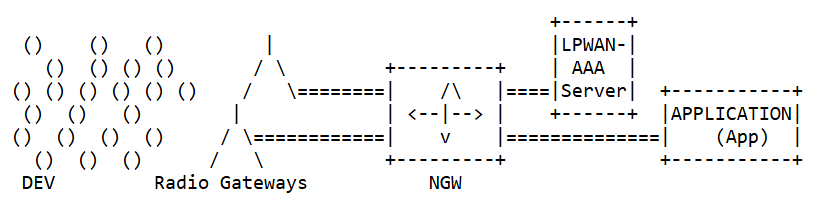
\includegraphics[width=400pt]{images/network.png}
		\caption{LPWAN Architecture. Reproduced from RFC8376 \cite{rfc8376}}
	\end{figure}

	\par{
		Given that the radio gateway marks the end of the constrained link we have it that all SCHC operations occur between the DEV and the NGW \cite{rfc9011, rfc8724}.
		Moreover, because of the network's star topology 
		the NGW is expected to store the SCHC configurations for all the DEVs connected to it,
		while each DEV only needs to store configurations that are directly assosiated with it's link to the NGW. A consequence of this 
		is that any operations made to update the SCHC configuration should occur at the NGW which then communicates the changes
		to the DEVs.
	}

\section{Compression}
	

	\par{
		The SCHC protocol uses a lossless, context based compression mechanism, that is, it makes use of previous knowledge
		about a given communication to omit repeated parts of a packet's metadata. Though it
		differs from other context based compression protocols in the derivation of said contexts,
		in which contexts are acquired in a purely offline and manual manner, relying on the network admins assumed
		pre-existing knowledge on the state of the communication between two endpoints to predefine the rules needed.
		This assumption is not only safe given the stable and simple nature of IoT applications with devices often running a single application, but
		also plays an important role in bypassing the need for synchronization messages. To put it into perspective, the minimum size of the metadata in a 
		COAP/UDP/IPv6 network stack is $\approx 60 \ bytes$ per packet, assuming the network stack is operating over a low data rate
		LoRaWAN connection
		means that the MTU would be 59 bytes with only 51 bytes available for application data \cite{lora_regional_params_2016},
		thus requiring fragmentation. 
		The additional overhead incurred by the need to fragment uncompressed packets in itself makes flow based context synchronization, similar to that used in the ROHC protocol unideal \cite{GomezMontenegro2020IPv6}.
	}

	\vspace{5pt}
	\par{
		Though even with predefined configurations, a compressor needs to first decide on which context to use based on the current network traffic before initiating
		the compression process.
		To best understand how a context rule is chosen, it is beneficial to cover the hierarchical structure of SCHC contexts.
	}

	\subsubsection{Context}
	A context in SCHC (also refered to as profile) is a pair $C = (CID, \ R)$ in which the CID is a unique identifier for the 
	devices connected to the NGW, used to decide on which context to use based on the DEV at the other end of the communication. The SCHC standard 
	puts no restrictions on what can be used as a CID and provides the option to use the DEV's data-link address (ie: MAC address). R on the other hand
	is a set of compression rules that can be used for the communications with the DEV that the CID corresponds to. 

	\subsubsection{Rules}
	SCHC rules can be thought of as blueprints for packet headers with some predefined field values. Each rule is represented as a pair $r = (RID, \ F)$ in which RID is a unique rule ID with it's uniqueness being
	in reference to the NGW's network and by extension all the DEVs connected to the NGW. While F is a set of field descriptors that dictate the expected 
	value that a field should contain, as well as the method in which fields are checked for the expected values and how to compress
	them if the check is sucessful.

	\subsubsection{Field Descriptors}
	Finally, A field descriptor is a 7-tuple $f= (FID, \ FL, \ FP, \ DI, \ TV, \ MO, \ ACT)$ in which the FID is an identifier for the 
	field's type (ie: IPv6 source address, UDP checksum, etc), FL refers to the size of the field in bits, FP is a position identifier used to
	distinguish between fields that repeat in the same header (ie: CoAP Uri-Path), DI is the direction of the packet as referenced in 
	section 2.1, TV is a set of target value(s) that the field is expected to have (can either be a single value or a vector), MO is a comparison operation performed
	on the field and the TV to decide if compression is allowed, and ACT is the compression and decompression action to perform on the field.


	\subsection{Packet Classification}
	Packet Classification refers to the process of determining the subset of rules that a packet can be compressed by. The compressor
	iterates over all the rules in the chosen context, and for each rule it 
	first performs a set of general checks that do not require looking into the content of the packet's fields, once the rule passes all
	the general checks we can then perform the matching operation which requires a deeper level of inspection on the packet's header.	

	\subsubsection{General Checks}
	The compressor begins by ensuring that for every field in the packet's header there exists a corresponding field descriptor with a matching FID.
	It then checks that the matched field descriptors have a DI value that matches the traffic direction, that is, it is 
	either set to ``UP" for up-link traffic, ``DW" for down-link traffic or "BI"
	for all traffic directions. Finally, the compressor checks for the existence of repeated fields in the packet's header, this check
	involves looking into the FP value of the matched field descriptors, if FP is set to 0 then the existence of repeated fields is not
	considered, thus all repeated fields are matched to the same field descriptor. On the other hand if there exists a field descriptor
	$f\ | \ f[FP] = j >0$ then there must exist a $j^{th}$ repeated instance of the field in the packet's header.

	The SCHC standard requires that a rule passes all the general checks, thus at any point when a check fails that rule is immediately
	disregarded and the compressor moves to checking the next rule in the context.

	\subsubsection{Matching Operations}
	Once a rule passes all the general checks, we will have it that every field in the packet's header will be matched to an appropriate
	field descriptor in that rule. Now for every field and its matched field descriptor, the compressor will apply the matching function
	defined by the descriptor's MO value on both the field and the descriptor's target value(s). SCHC defines 4 of matching functions
	that the field descriptor can use:
	
	\begin{itemize}
		\item \textbf{Equal:} A direct equality comparison between the field's value and the descriptor's TV; requires the TV to be a single value.
		\item \textbf{Ignore:} No comparison is performed, always returns True.
		\item \textbf{MSB(x):} The compressor compares the $x$ most significant bits in the field against the TV; requires the TV to be a single value.
		\item \textbf{match-mapping:} Checks if the field is \textbf{Equal} to any of the values stored at the TV; requires the TV to be a vector.
	\end{itemize}
	
	Note that the SCHC standard makes no further restrictions on rule selection beyond the aforementioned checks; observe that applying both the 
	general checks and the matching operations does not guarantee
	that only a single rule is valid. Thus different implementations might want to test all the rules in the context first then choose one
	with the highest compression ratio such as those with highly constrained links, while other implementations might prefer to short circuit the checking process and choose the first matching
	rule when. 
	

	\subsection{Compression/Decompression Modes}
	Before discussing SCHC's compress process, we must first cover the different compression functions (often referred to as
	actions) that the standard defines. Compression functions in SCHC can either completely omit a field, in which the compressor
	avoids transmitting the field, knowing that the decompressor knows what that field's value is based on the compression rule used, or
	the compression function may replace the field with a different (often smaller) value called the field residue which will be sent 
	to and used by the decompressor to derive the original field. The 7 actions defined by the standard are:
	\begin{itemize}
		\item \textbf{not-sent:} At compression the field is completely omitted with no residue produced. The decompressor uses the TV stored
			in the rule as the field's value.
		\item \textbf{value-sent:} The field is not compressed, instead it is fully sent as a residue and used by the decompressor as is.
		\item \textbf{mapping-sent:} This action occurs in conjunction with the match mapping MO, in which the compressor
			sends the index of the field's value as found in the TV vector. The decompressor then uses the index to retrieve the value from the TV
			vector.
		\item \textbf{LSB:} Again, this action is only used in conjuncture with the MSB(x) MO, in which the compressor send the field's
			$f[FL]-x$ least significant bits as residue, which the decompressor prepends with the MSB stored in the descriptor's TV.
		\item \textbf{compute:} This action is kept for fields used in integrity checks (ie: UDP checksum), in which the output of the 
			integrity check (often a hash value) is used as the field residue.
		\item \textbf{DevIID and AppIID:} Both these actions serve the same purpose in which the compressor omits the 64 least significant
			bits in either the DEV's or the NGW's IPv6 address resp. for DevIID and AppIID. The decompressor uses the data-link layer address
			as the IID (interface identifier)
	\end{itemize}

	\subsubsection{Field Residue}
	We mentioned that certain compression functions produce field residues that are required by the decompressor to derive the original
	field value, one caviat of using a system of residues is their need for additional metadata in cases when the residue size is variable,
	this occurs when using the value-sent or compute actions. In this case the compressor must prepend the residue with it's size which
	is encoded as either a 4 or 12 or 28 bit 2's complement integer, with the encoding being dictated by the descriptor's $f[FL]$ value.
	\subsection{Compression}
	Given a compression rule and a packet header, the compressor begins by creating a new \textbf{compressed}
	packet and prepending the selected rule's RID to it
	. It then iterates over all of the rule's field descriptors based on their order in the rule definition, for every field
	descriptor we apply the compression function (dictated by the descriptors $f[ACT]$ value) on both the field's value
	and the descriptors TV. In the case where the compression action returns a residue, we append it to the \textbf{compressed} packet,
	otherwise move on to the next field descriptor. Figure 2.2 represents the final compressed packet.

	\begin{figure}[h]
		\center
		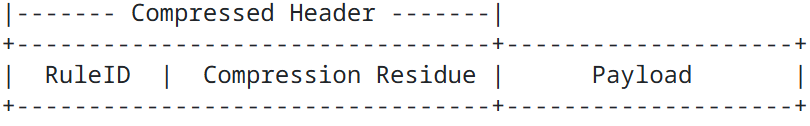
\includegraphics[width=300pt]{images/schc_pkt.png}
		\caption{SCHC compressed packet. Reproduced from RFC 8724 \cite{rfc8724}}
	\end{figure}

	\subsection{Decompression}
	The decompression process is a simple inversion of the compression step. The decompressor begins by reading the RID at the 
	start of the compressed packet, which points it to the rule used, it then iterates over the rule's field descriptors in the order
	that they are defined in (just as in compression). For every descriptor with an $f[ACT]$ that produces a residue the decompressor
	reads in the next residue block from the compressed packet and uses it in the decompression action defined by the descriptors $f[ACT]$
	value.
	
	\subsection{Compression Ratios}
	SCHC's compression framework has the capability of producing large compression ratios, with studies reporting
	ratios of around 45\% - 54\% decrease in the size of \\CoAP/UDP/IPv6 headers as well as a 76\% - 95\% decrease on CoAP/UDP headers \cite{Tomoskozi2022Packet}. We 
	observe however that these compression ratios are unilaterally dependent on the quality of the SCHC rules at predicting the 
	application's packets. Take for example the case of a stationary sensor that has the sole purpose of pinging 
	a server with a CoAP POST request with the current temperature, given knowledge of the
	endpoints IP addresses and the exact application running on them, a user is able to define SCHC rules with the IPv6 address, UDP ports and 
	CoAP methods being predefined.
	Thus the output of compression need only contain the RID, integrity checks and payload. This means that a header
	with minimum size of 60 bytes can now be represented in as little as 3 bytes + payload. On the otherhand, any uncertainty 
	regarding the endpoint's IP addresses can result in the transmission of those fields uncompressed (as a residue), resulting in the compressed header
	to have a minimum size of 35 bytes + payload.


\section{Mobility Limitations of SCHC}
		While SCHC has demonstrated the capacity to provide impressive compression ratio's when provided with a 
		comprehensive rule set, it's dependence on the presistence of the network's state comes with major drawbacks - mainly it's inability 
		to adapt to certain changes in network configurations that may occur between the DEV and the NGW. 


		Take for example the use of SCHC in a communication in which the IoT device is mobile and moves between different
		networks.
		While existing standards such as MIPv6 (Mobile IPv6) may be used to ensure that IoT devices
		keep their IP addresses even when moving between networks, and thus maintaining their context. The use of such
		protocols in low power IoT devices is currently infeasible given the long hangover latency, intense signaling and packet loss attributed to them 
		\cite{Ghaleb2016}. 

		That is to say, we have proof of the advantages of applying SCHC to mobile based IoT applications such as that demonstrated by
		\cite{8355231} however the actual deployment
		of SCHC into applications with changing network configurations 
		comes at the cost of lossing the ability to compress large part's of the packet, such as 
		the source and destination IPv6 addresses which are by definition variable in these use cases.

\chapter{DYNAMIC RULE UPDATING}
	\section{Previous Work}
	\par{
		The idea behind using dynamic context synchronization is not novel, and was mention by \cite{Tomoskozi2022Packet} in their survey of 
		header compression protocols with reference to learned or negotiated context exhanges as well as the posibility of bootstrapping SCHC
		dynamicly using context registration. Further, the groundworks for exchanging contexts have already
		been 
		developed with existing SCHC implementations such as openSCHC including mechanisms to convert SCHC contexts into the YANG data model which
		can then in turn be compressed via CBOR, and transmitted via the SCHC channel uncompressed (though fragmentation
		is likely required).
	}

	\section{Algorithm}


	\par{
		With the excesive overhead of flow based rule updating of ROHCv1 \cite{GomezMontenegro2020IPv6} (as mentioned in sec 2.2) and the 
		relativley high computational complexity of ROHCv2 via it's context state machine, relative to LPWAN networks \cite{Tomoskozi2022Packet}. 
		It follows then that given the existance of context exchange mehanisms, what remains is simple algorithms that operate in the bounds of SCHC's network
		architecture to decide on which rules to use as well as the frequency
		of updating the rules. 
	}


	\par{
		On a high level the procedure can be thought of as a continuos transition between two states that is occuring at the NGW, an initiating state where 
		no dynamic updating is yet to take place with
		either static rules being used or no compression, and an update state
		which is transitioned to after the first update and repeats indefinitly to continue updating the rules as per the update frequence parameter.
	}

	\begin{center}
		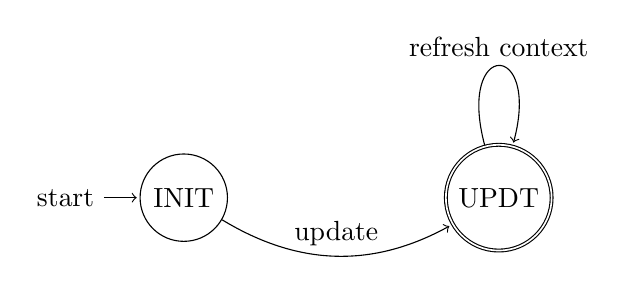
\begin{tikzpicture}[shorten >= 1pt, node distance=4cm, on grid, auto]
		\node[state, initial] (q_0) {INIT};
		\node[state, accepting]					(q_1)	[right=of q_0] {UPDT};
		\path[->]
			(q_0) edge[bend right] node {update} (q_1)
		(q_1) edge[loop above, looseness=10] node {refresh context} (q_1);
	\end{tikzpicture}
	\end{center}

	\subsection{Weight assignment}
		\par{
			Given SCHC's network architecture (in section 2.1) we have it that all traffic passes through the NGW, thus for every packet
			that passes through the NGW a weight is assigned to the header fields which will then be used in predicting the compresion rules.
		}
		\par{
			The NGW maintains fixed sized priority queues for every field we wish to dynamically update, in the case of mobile networks the source and destination
			IPv6 addresses are sufficient since the remaining fields are not affected by mobility. The entries in each queue corresponds to a 3-tuple (P, [ID], value)
			where value is the IP address, ID is a list of identification values we assign to packet flows, and P is the priority value.

			The NGW also defines two variables, an update and aging frequencies resp. which
			dictates the number of packets that are forwarded by the NGW between the DEV and APP pair before a rule update should occur,  and 
			 before the priority values in the queue are aged (decreased) allowing for more adaptive responses to network changes.
		}

		\par{
			For every packet that the NGW recieves it checks the source and destination address, packets with the same source and destination addresses
			are assigned the same ID. After parsing the packet the priority queues are updated by increasing the priority of the entry with the 
			respected address as value (or adding it if it is not in the queue) and updating the list of IDs for the specified address.
		}

		\par{
		Finally, the frequency parameters are checked to either trigger queue aging or rule updates.
		}
		
		\subsection{Choosing Rules}
		\par{
			Once the update frequency parameter triggers a rule update the follows steps take place: 
		}

		\par{
			First, the $x$ packet flows (by ID) with the highest cummulative priority value across all the queues are selected
			, these will be
			the top level compression rules in which there will be a new rule  for each flow, with the \textbf{not-sent} compression action being used for the
			specified fields, allowing for maximum compression of both the source and destination addresses.
		}
		\par{
			Next, find the $y$ top queue entries by priority that do not share an ID with any of the $x$ top level rules. Once $y$ values 
			are selected from each queue, a set number of second level rules are created in which subsets of the chosen $y$ values are 
			grouped together in their corresponding field descriptor's TV with the compression action being set to \textbf{match-mapping}
			thus partial compression occurs with the index of the address relative to the TV being sent as field residues.
	}

	\subsection{Rational}
	\subsubsection{Assumption}
	\par{
		An explicit assumption made while defining the rule update procedure is that of a reasonable levels in variability. So
		while the expected traffic that SCHC operates on is expected to be mostly presistent, the update procedure still assumes some level of 
		stability in the type of traffic but loosens the requirement to allow for some variability.
	}

	\subsubsection{Explaination}
	\par{
		By assigning the top $x$ flows their own rules with the maximum compression ratio possible we make it so that
		the most frequently sent packets have the smallest size. On the otherhand by assigning the $y$ second level fields
		rules with index matching, we make it so that less frequent but still used packet fields are also compressed, be it at a slightly lower compression
		ratio.
	}

	\par{
		The main reason for the distinction between the top $x$ and $y$ values is aimmed to limit the total number of rules used. Each 
		rule represented in YANG format and compressed by CBOR is $\approx 400$ bytes thus we want the updates to be small and less frequent. Further, more
		rules means that a larger number of bits is required to uniquley assign RID values. Similarly a limit on the number of
		$y$ values per TV vector is desirable to restrict the number of bits needed to index the TV vector.
	}

	\par{
		
	}
	\chapter{METHODOLOGY}
	\section{Testbed and Workflow}
	All tests are performed in an emulation environment provided by the OpenSCHC Virtual Machine running
	the openschc python implementation of the SCHC standard. The general testing architecture includes three devices, a DEV representing
	the low-power IoT device, a NGW representing a LPWAN network gateway, and an external CoAP server. 	
	
	The tests emulate down-link traffic flowing in two stages,
	first uncompressed CoAP packets are transmitted from the server to the NGW. The NGW then
	runs the dynamic updating algorithm and performs SCHC compression on the packets that are then dispatched to the DEV.  
	Finally the DEV decompresses the packets and reads their contents to ensure correct compression and decompression. 

	\section{Dataset}
	To test the performance of dynamic updating based on the different levels of network variability, we need to have direct control
	over the distribution of packets that are being transmitted. To do this we define a sample space $S$ as a set of 80 randomly generated CoAP/UDP/IPv6 
	packet headers each sized between $57-64$ bytes. 
	We then sample 10000 packets from $S$ with replacement using two samplinging distributions: 
	\begin{itemize}
		\item \textbf{Dataset A:} A heavily skewed and narrow beta distribution with $\alpha = 2, \beta = 40$ and a $\sigma \approx 0.05$ .
		\item \textbf{Dataset B:} A less skewed beta distribution  with $\alpha = 10, \beta = 10$ and a $\sigma \approx 0.48$. 
	\end{itemize}

	Dataset A simulates a stable network with little to no variability in the header fields of the pakets being transmitted.
	Dataset B simulates a slightly more variable network as we increase the standard deviation.

	\section{Evaluation}
	\subsection{Control Group}
	\par{
		For every dataset we begin by filtering out the $x+y$ most repeated packet headers and create static rules for them with the compression action
		set to \textbf{not-sent} allowing for maximum compression. We then transmit the packets from the APP to the NGW and log the original vs compressed
		size of every packet. 
	}

	\subsection{Dynamic Updating}
	\par{
		To evaluate the performance of the rule updating procedure, we begin by setting the NGW to the initiating state with no static compression rules
		defined, we then transmit the dataset packets from the APP to the NGW, the NGW performs the rule updating procedure then attempts
		to compress the packets, logging the size of the original and compressed headers. Finally the compressed packet is transmitted to the DEV.

		Whenever a rule update is triggered the NGW also logs in the size of the context's CBOR representation which needs to be transmitted for 
		the update to occur, and
		thus counts as a penalty cost for perfroming an update.
	}


	\chapter{RESULTS AND ANALYSIS}
		In this section we focus on comparing the size, in bytes, of the compressor's output traffic, flowing from the NGW to DEV for each of 
		the datasets on both the Control (static) and dynamic implementations of SCHC rules. 

		\section{Direct Comparision}
		By analysing the running average of the size of packets flowing from the NGW to the DEV (the compressor's output) in figures 5.1 and 5.2. We first
		observe that the average size of compressed headers for the control (static) implementation on datasets A and B differ by $\approx 10$ bytes 
		this confirms our initial analysis on the static rule's performace being heavily dependanant on the stability of the network traffic, that is, the 
		static rules performed considerably better with lower levels of variability in the packets sent.

		On the otherhand, the dynamic rule updating showed a possitive correlation between imporvemented compression ratios and the number of 
		packets being compressed, indicating that the updating hueristics perform well for both distributions.
	
		\newpage
		\begin{figure}[H]
			\centering
			
\includegraphics[width=350pt]{images/b40a2.png}
			\caption{Running average of compressed header size on Dataset A}
		\end{figure}
	
	\begin{figure}[H]
			\centering
			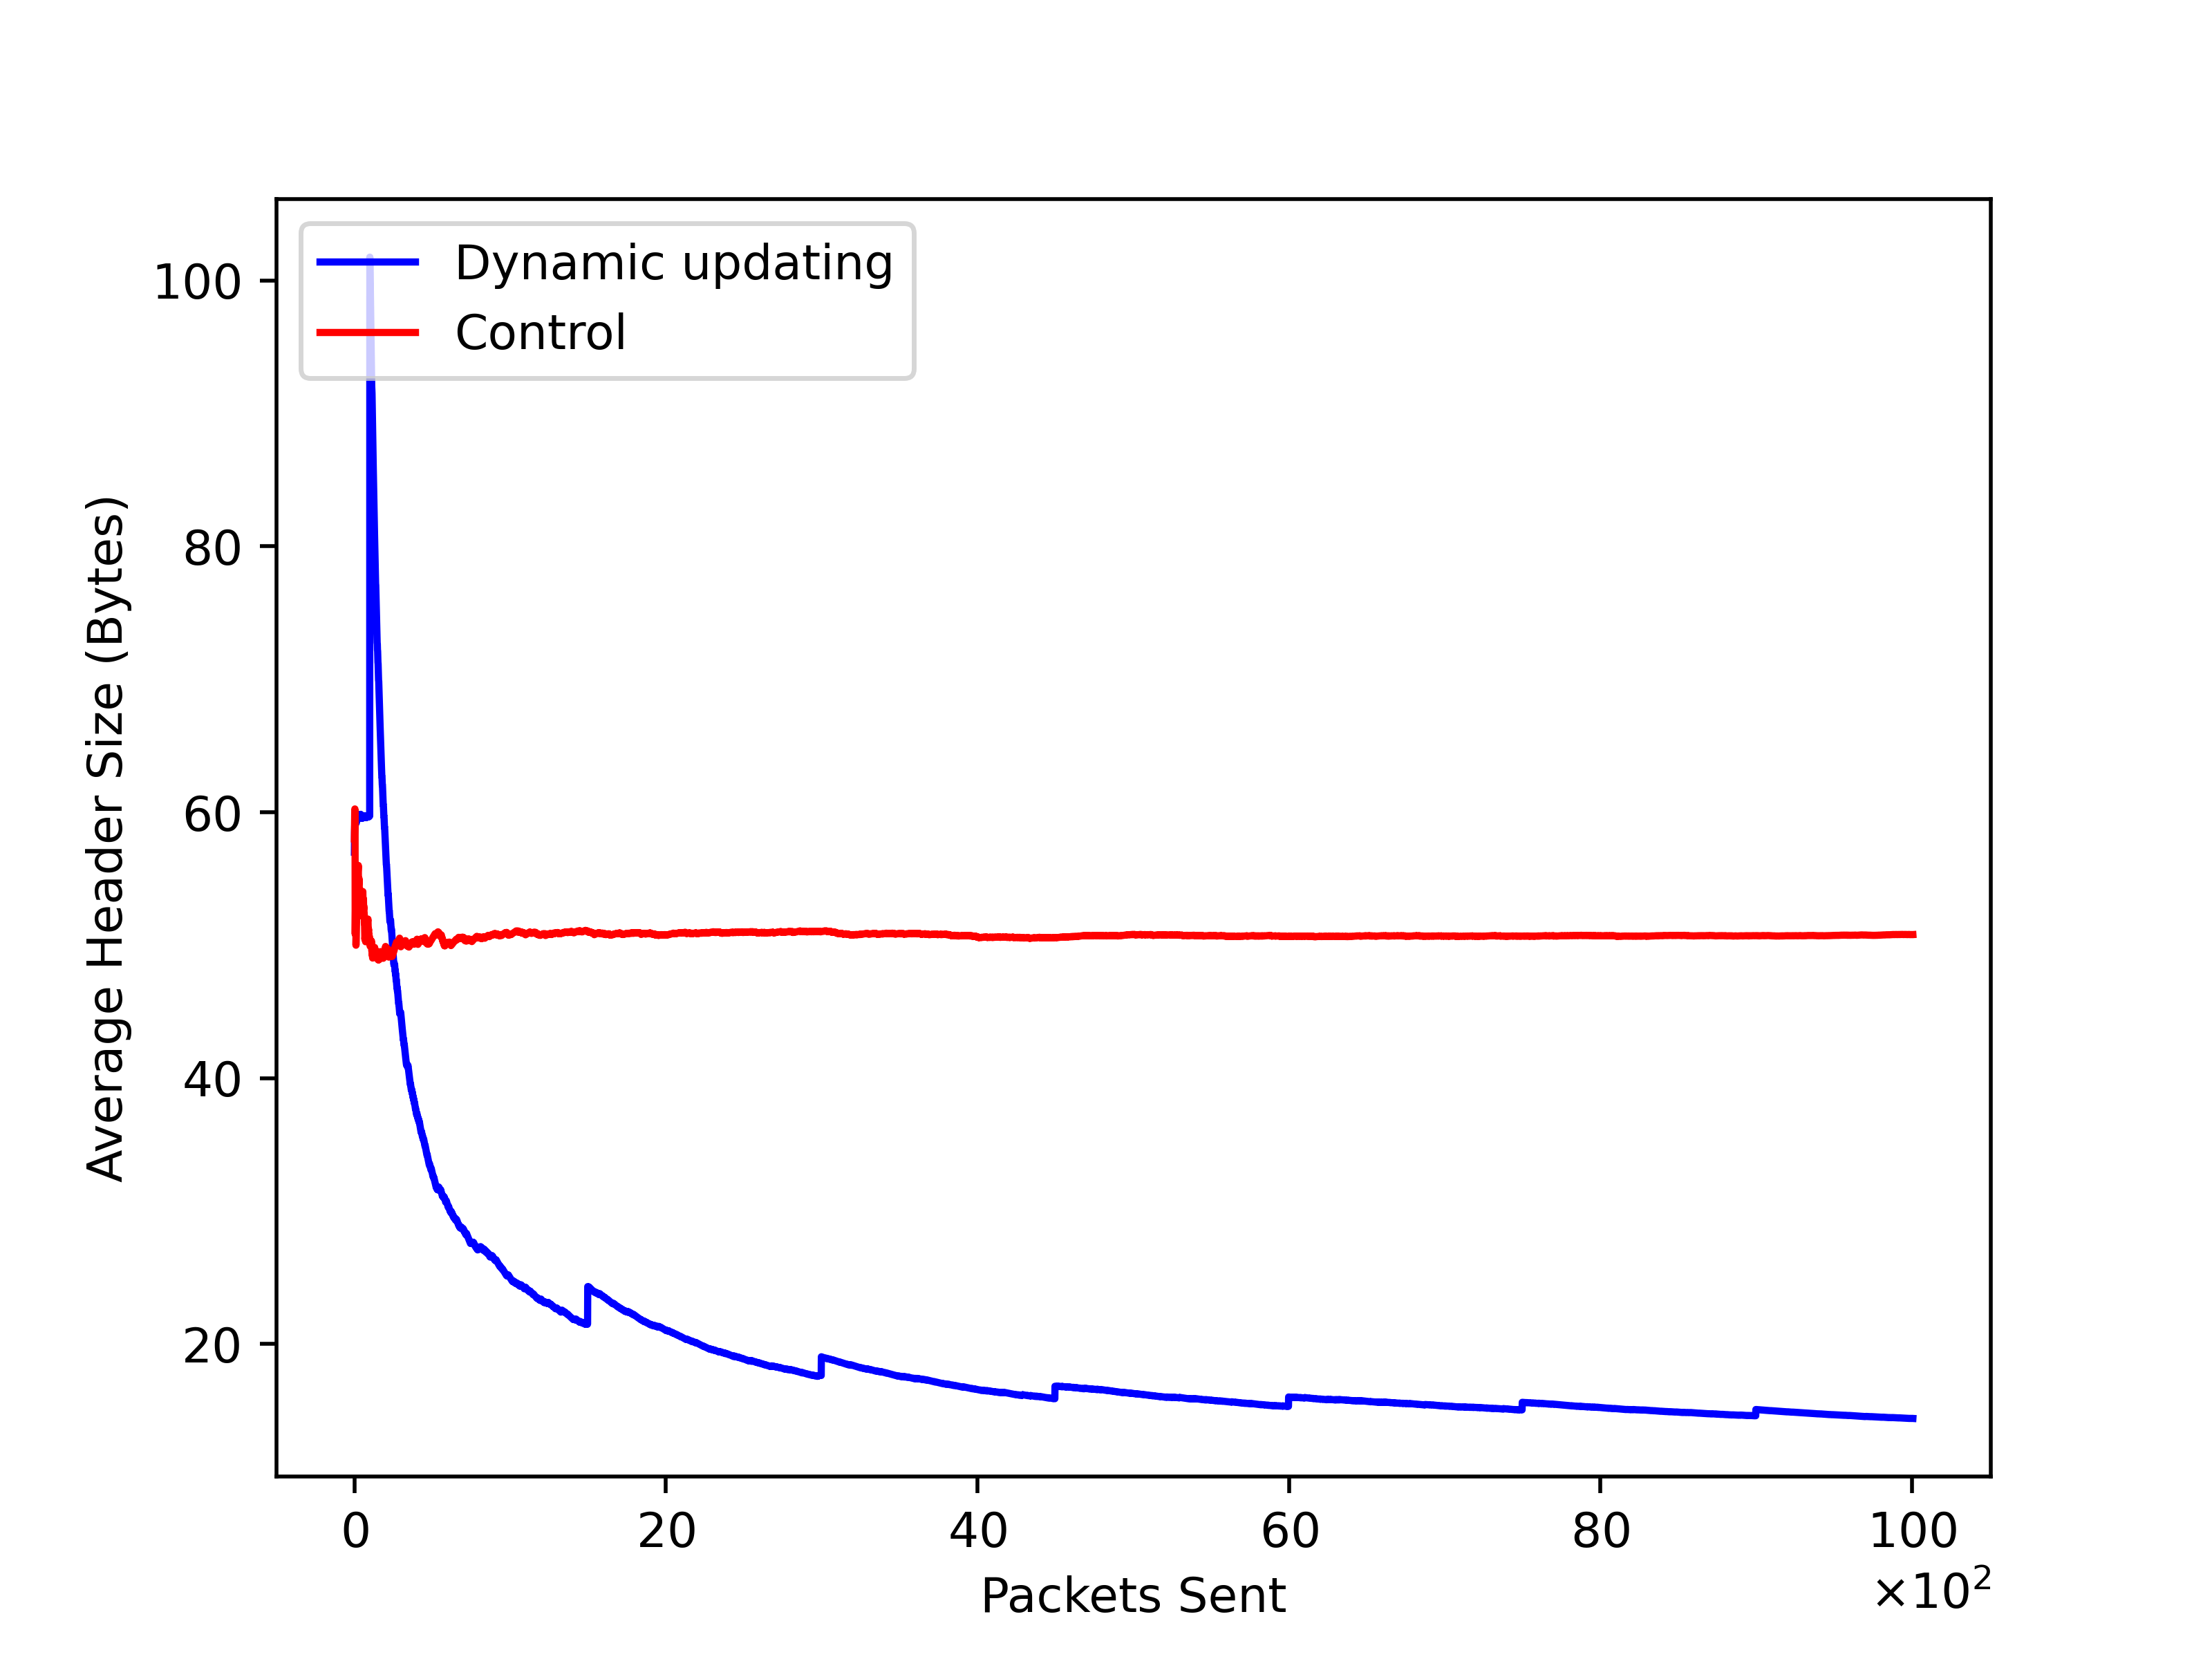
\includegraphics[width=350pt]{images/b10a10.png}
			\caption{Running average of compressed header size on Dataset B}
		\end{figure}

		
		\newpage
		\newpage
		\section{Limitation}
		While the use of the rule updating procedure showed significant decrease in the average packet size. This came at the cost 
		of large occasional spike as seen in the initial surge in Figures 5.1 and 5.2. 

		Moreover, the surges in header size become more aparent when instead of a running average we group packets into 
		windows of size 10 and calculate the average size of the headers in each window, as seen in Figure 5.3. 
	
	\begin{figure}[H]
			\centering
			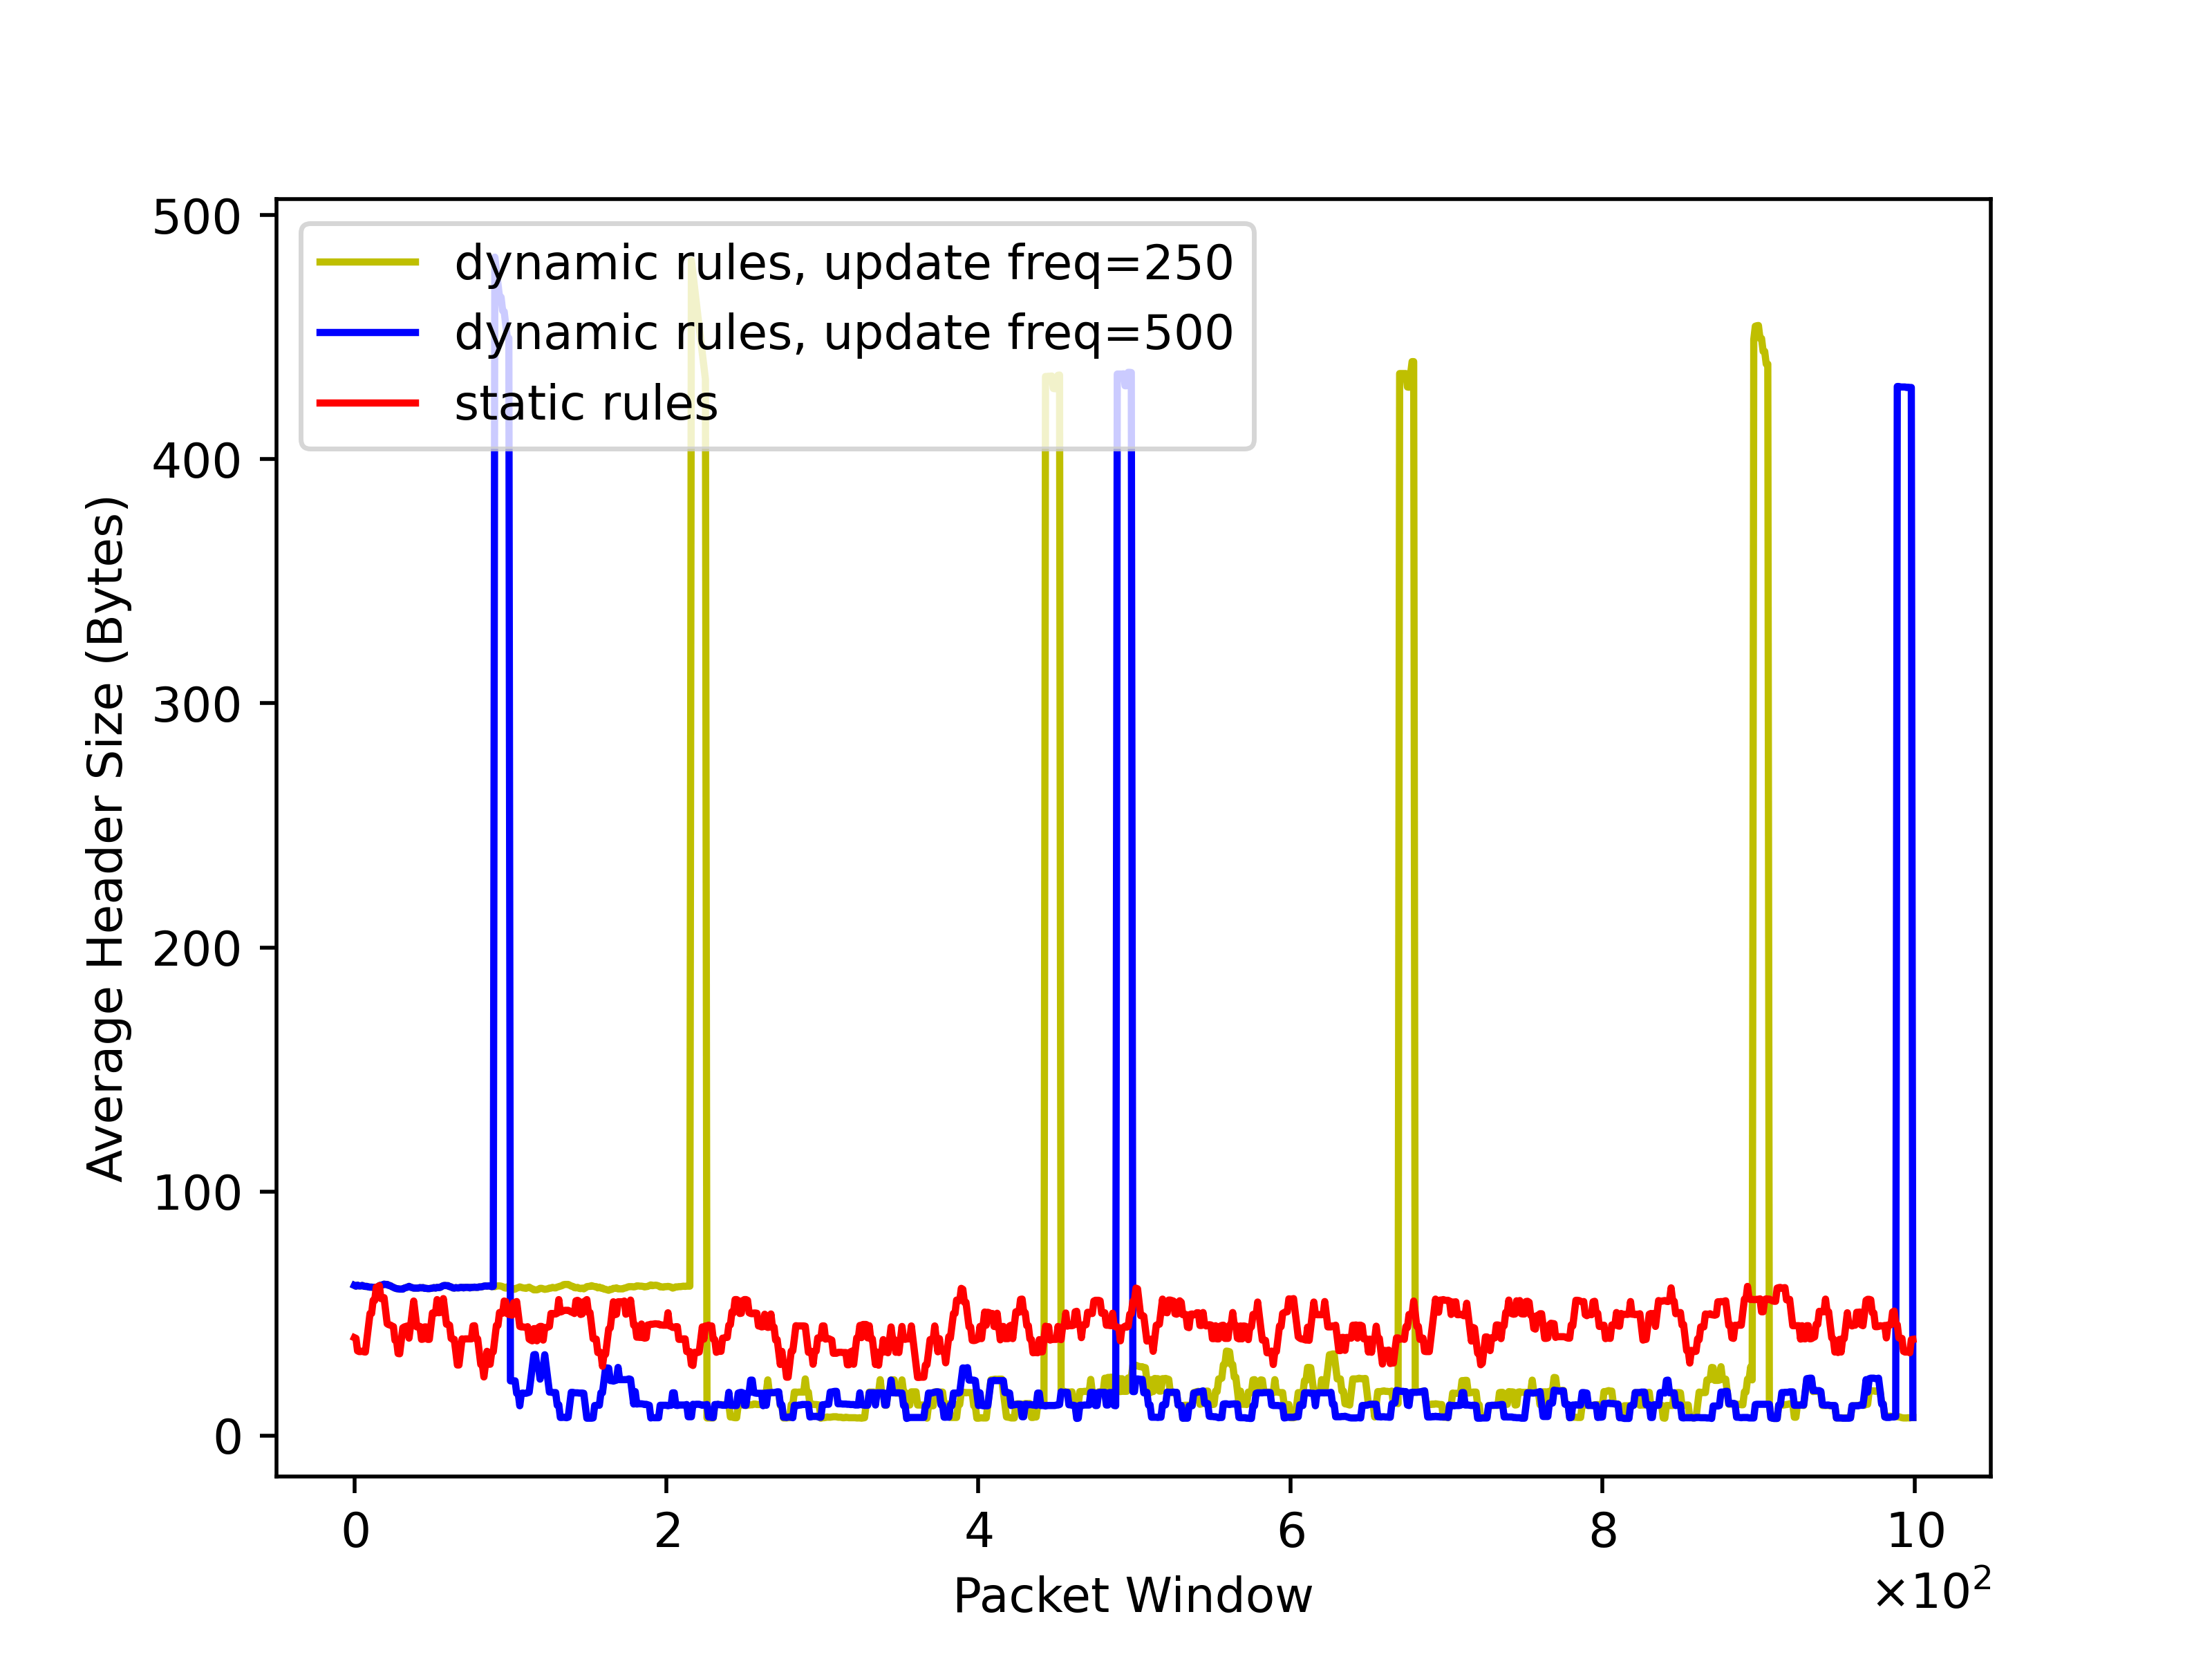
\includegraphics[width=400pt]{images/windowed_average.png}
			\caption{Windowed average of compressed header size on Dataset A}
		\end{figure}

	

		We note here that the extreme spikes seen in Figure 5.3 represent failed rule updating, in which a rule synchronization packet is 
		sent from the NGW to the DEV to update the rules, however the next window of packets breaks from the trend that dictated the new rules.
		The probability of these spike and the frequency of updates naturaly has a positive correlation. 

		While only 3 such spikes occured over a 10000 packet exchage, the extremley constrained nature of LPWAN networks may not be able to
		efficiently deal with them, as such careful assessment on the nature of the constrained link should be performed to ensure that 
		spikes in header size do not become a choking point for the connection.

\chapter{Conclusion}
	\section{Summary of Contribution}
	This thesis introduces the SCHC protocol's compression framework which is considered to be 
	at the cutting edge of header compression in the context of LPWAN networks and highlight rational and assumptions behind certain aspects of 
	it's design with regard to context sharing. We then raise some of the concers regarding the deployment of SCHC in mobile networks and introduce a
	simple mechanism as a proof of concept for the possibility of integrating dynamic context updating which should make the use if SCHC in 
	mobile and other inheritly unstable networks with prospected IoT applications.

	\section{Possible Improvements}
	The current implementation of the rule updating presented in this thesis, while was able to show the possible benifits of dynamic rule updating
	also proved to be too simplistic in nature that it repeated some of the issues and limitations facing the previously mention RoHC (Section 2.2).
	
	Moreover, the deployment of rule updating outside of an emulation enviroment would require additional mechanisms the deal with illformed and missing
	rule synchronization messages, thus the development and testing of 
	such mechanisms in a deployment enviroment is necessary in gauging the perfromance of rule updating. 

	\section{Future Work}
	The utilization of simple refinforcement algorithms based on the network traffic as opposed to weight and scheduling heuristics may be an interseting
	pivot when considering the process of creating new rules. Moreover, given that SCHC is both a compression and fragmentation protocol, it would
	be benificial to test the impact of rule updating in selecting fragmentation rules, especially in relation to the different acknoledgement 
	modes that SCHC fragmentation uses.

	\bibliographystyle{plain}
\bibliography{thesis}

\end{document}

